% Geometry, font
\documentclass[12pt, letter]{article}
\usepackage[margin=0.8in]{geometry}
\usepackage[T1]{fontenc}
\usepackage{fourier}
\usepackage{titling}
\setlength{\droptitle}{-5em} 
\usepackage[parfill]{parskip}
\usepackage{graphicx}
\graphicspath{{imgs/}}
\usepackage{hyperref}

\usepackage{fancyhdr}
\lhead{ECE 4542: Advanced Engineering Algorithms}
\rhead{Zach Neveu}
\pagestyle{fancy}

% Math stuff
\usepackage{amssymb}
\usepackage{bm}

% Code Highlighting
\usepackage{minted}
\usemintedstyle{solarizedlight}

\title{ Homework 2 }

\begin{document}
\maketitle
\thispagestyle{fancy}

\begin{enumerate}
	\item 3.2-3
\begin{minted}{Python}
# Model File
var x1 >= 0, <= 1;
var x2 >= 0;
 
maximize Z:
    4500*x1+4500*x2;
 
subject to c1:
    5000*x1+4000*x2<=6000;
 
subject to c2:
    400*x1+500*x2<=600;

# Solution
MINOS 5.51: optimal solution found.
3 iterations, objective 6000
x1 = 0.666667
x2 = 0.666667
\end{minted}

\item 4.1-1
\begin{itemize}
\item Graphical Solutions
\begin{figure}[h]
	\centering
	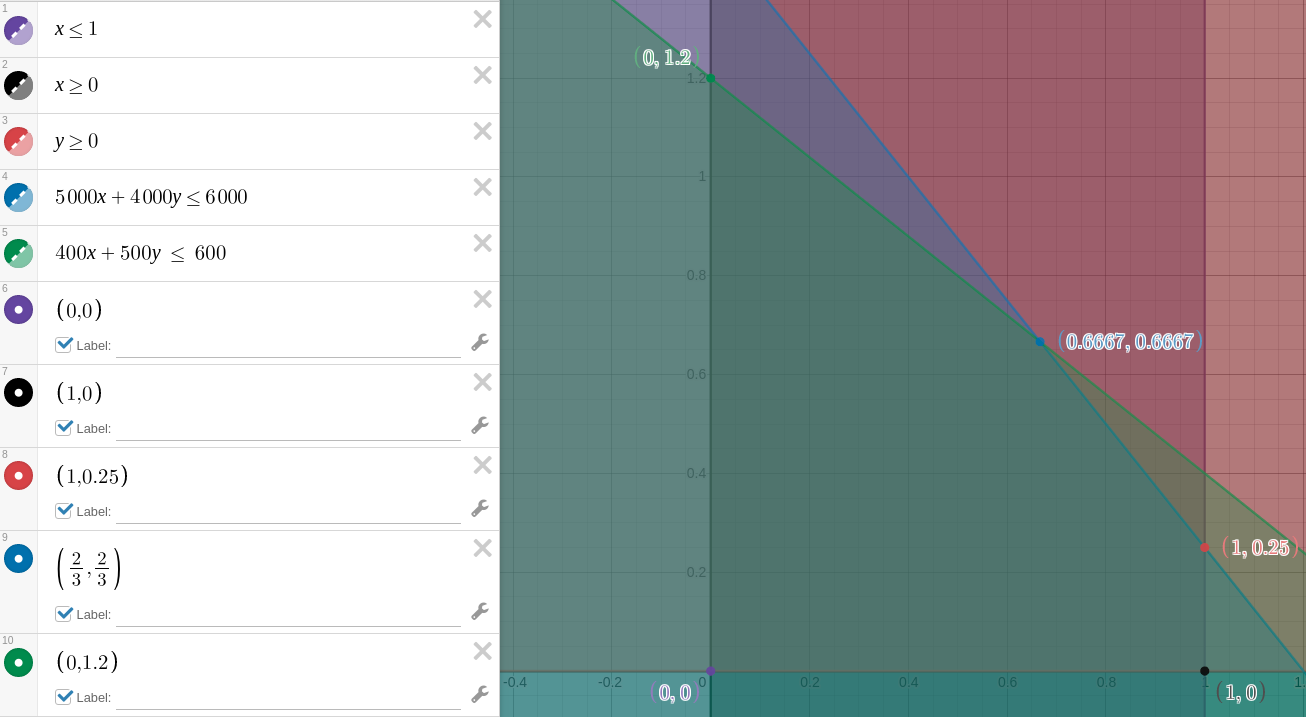
\includegraphics[width=0.8\textwidth]{p1a}
	\caption{Graphical Solutions}
	\label{fig:p2}
\end{figure}
\item Calculated Z Values
\begin{figure}[h]
	\centering
	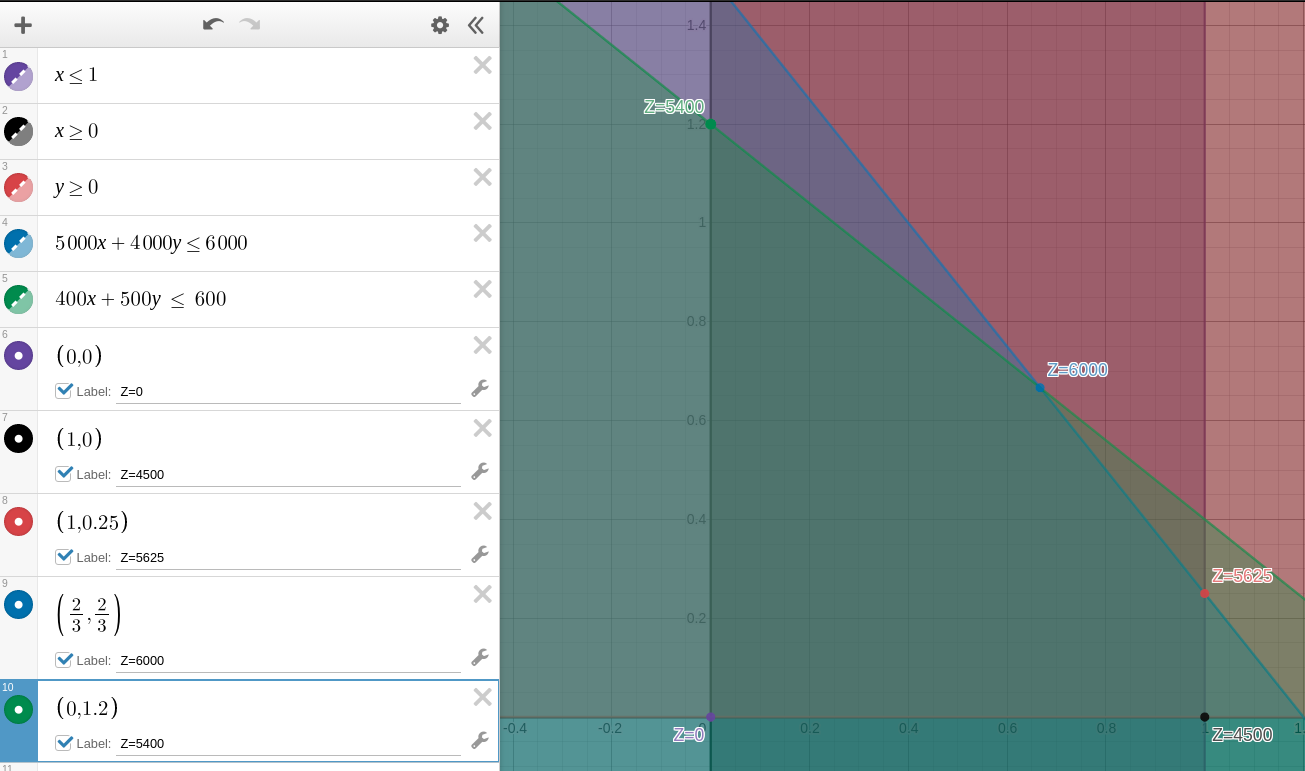
\includegraphics[width=0.8\textwidth]{p1b}
	\caption{Calculated Z Values}
	\label{fig:p2b}
\end{figure}
\item Simplex Method
\begin{itemize}
	\item Start at (0,0).
	\item Check for optimality - Fails
	\item Follow edge to (4/3,0)
	\item Check for optimality - Passes
	\item Optionally continue to (2/3, 2/3) depending on implementation
\end{itemize}
\end{itemize}

\item 4.1-2
\begin{itemize}
\item Ampl
\begin{minted}{Python}
# Model File
var x1 >= 0;
var x2 >= 0;

maximize Z:
    x1 + 2*x2;

subject to c1:
    x1 + 3*x2 <= 9;
subject to c2:
    x1 + x2 <= 4;

# Solution
MINOS 5.51: optimal solution found.
2 iterations, objective 6.5
x1 = 1.5
x2 = 2.5
\end{minted}
\item Graphical Solutions
\end{itemize}
\begin{figure}[h]
    \centering
    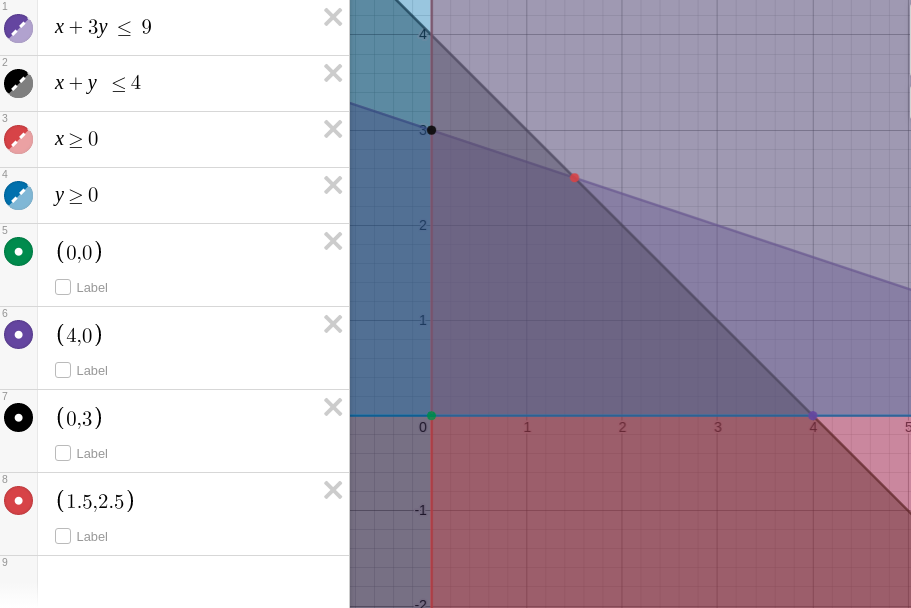
\includegraphics[width=0.8\textwidth]{p3a}
    \caption{Graphical Solution}
    \label{fig:p1a}
\end{figure}
\item Calculated Z Values
\begin{figure}[h]
    \centering
    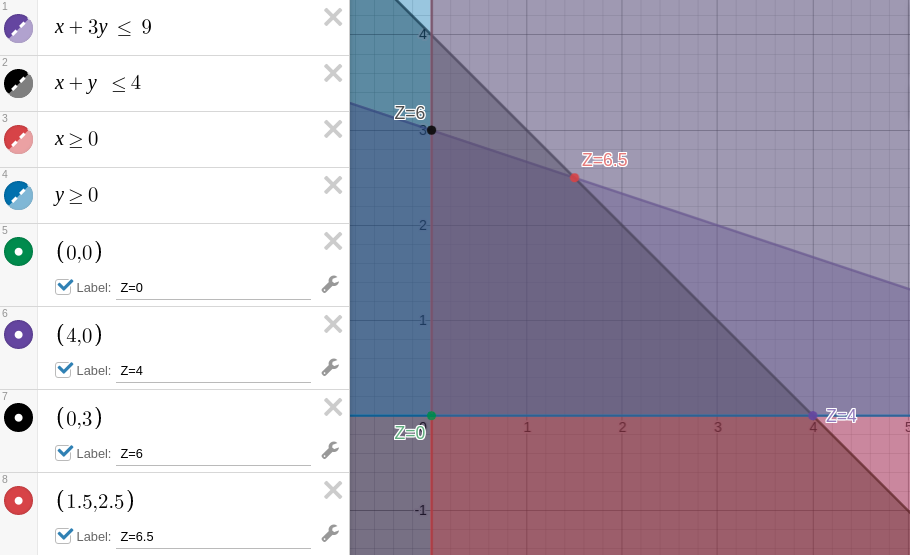
\includegraphics[width=0.8\textwidth]{p3b}
    \caption{Calculated Z Values}
    \label{fig:p1b}
\end{figure}
\item Simplex Method
\begin{itemize}
	\item Start at (0,0)
	\item Check for optimality - Fails
	\item Follow Edge to (0,3)
	\item Check for optimality - Fails
	\item Follow edge to (1.5,2.5)
	\item Check for Optimality - Succeeds
\end{itemize}

\item 4.1-3
\begin{itemize}
\item Ampl
\begin{minted}{Python}
# Model
var x1 >= 0, <= 4;
var x2 >= 0;

maximize Z:
	3*x1 + 2*x2;

subject to c2:
	x1 + 3*x2 <= 15;

subject to c3:
	2*x1 + x2 <= 10;

# Solution
MINOS 5.51: optimal solution found.
3 iterations, objective 17
x1 = 3
x2 = 4
\end{minted}
\item Graphical Solutions
\begin{figure}[h]
	\centering
	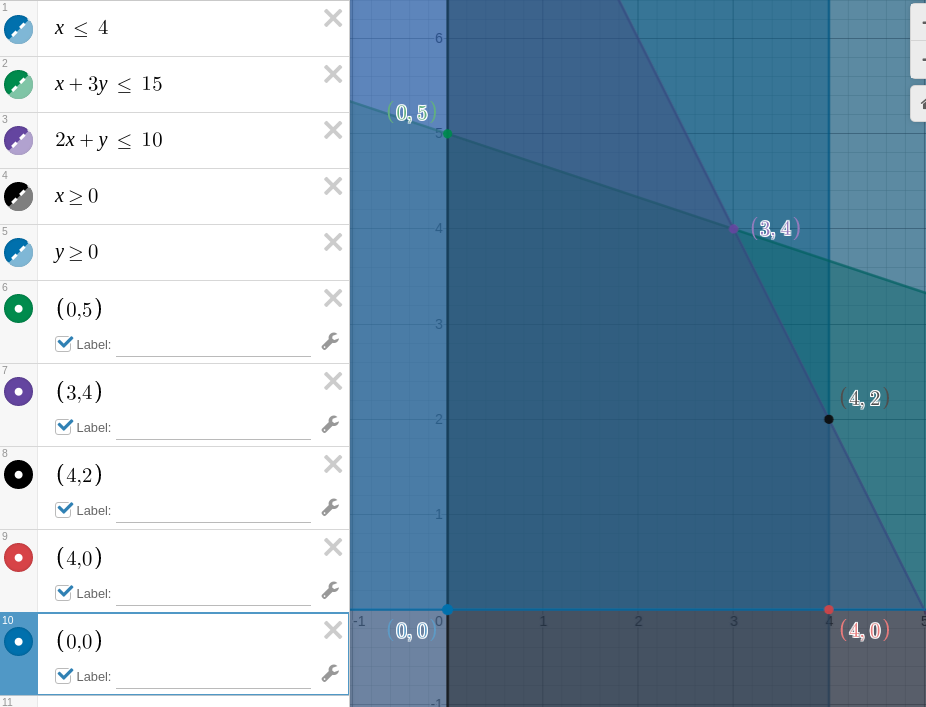
\includegraphics[width=0.8\textwidth]{p4a}
	\caption{Graphical Solutions}
	\label{fig:p4a}
\end{figure}
\item Calculated Z Values
\begin{figure}[h]
	\centering
	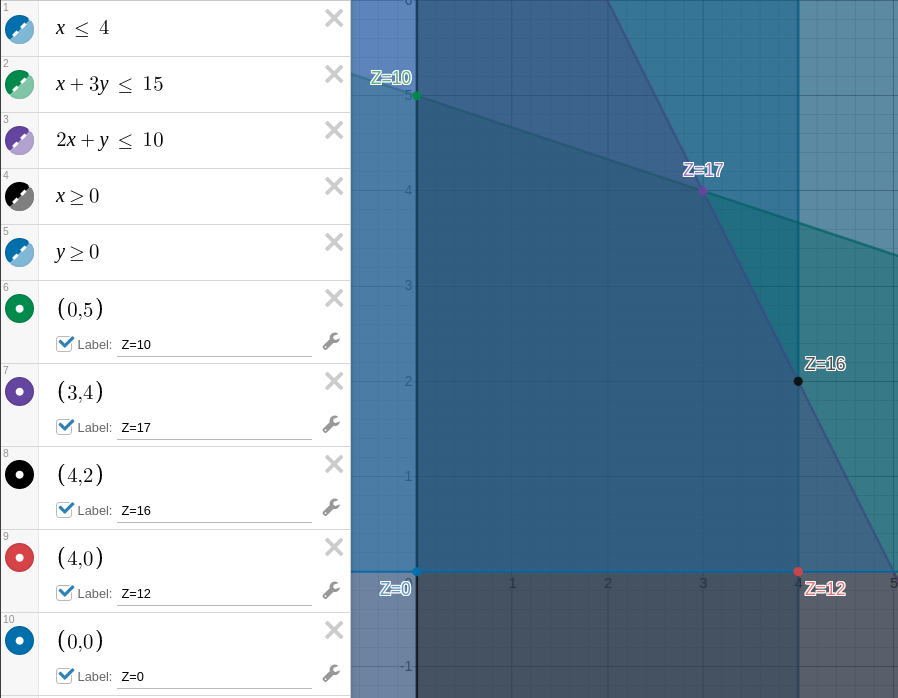
\includegraphics[width=0.8\textwidth]{p4b}
	\caption{Calculated Z Values}
	\label{fig:p4b}
\end{figure}
\item Simplex Method
\begin{itemize}
	\item Start at (0,0)
	\item Check for optimality - Fails
	\item Follow Edge to (4,0)
	\item Check for optimality - Fails
	\item Follow edge to (4,2)
	\item Check for Optimality - Fails
	\item Follow edge to (3,4)
	\item Check for Optimality - Succeeds
\end{itemize}
\end{itemize}
\item 4.1-4
\begin{enumerate}
	\item True - This is the definition of an optimal solution
	\item False - In certain cases every point along an edge could be optimal solutions.
	\item True - In the case where a constraint runs perpendicular to the Z function, this will be the case.
\end{enumerate}
\end{enumerate}
\end{document}
